\section{Compacidad}

\subsection{Espacios compactos}

\begin{definición}[Recubrimiento]
    Un recubrimiento de un conjunto $X$ es una familia de subconjuntos de $X$, $\mathcal{U} = \{A_i : i \in I\} \subset \mathcal{P}(X)$ tal que:
    $$\bigcup \mathcal{U} = \bigcup_{i \in I} A_i = X.$$
    Si el conjunto $I$ es finito, se dice que $\mathcal{U}$ es un recubrimiento finito.
\end{definición}
\begin{definición}[Recubrimiento abierto]
    Sea $(X, \tau)$ un espacio topológico, $\mathcal{U} = \{A_i : i \in I\}$ un recubrimiento de $X$ si los $A_i$ son todos abiertos, es decir, $\mathcal{U} \subset \tau$, se dice entonces que $\mathcal{U}$ es un recubrimiento abierto de $(X, \tau)$.
\end{definición}
\begin{definición}[Compacto]
    Un espacio topológico $(X, \tau)$ es compacto si todo recubrimiento abierto de $(X, \tau)$ admite un subrecubrimiento finito, es decir, 
    $$\forall \mathcal{U} \subset \tau : \bigcup \mathcal{U} = X, \exists \mathcal{V} \subset \mathcal{U} \text{ finito } : \bigcup \mathcal{V} = X.$$   
\end{definición}
\ejemplo{Algunos ejemplos son las topologías finitas, discretas, la de Kolmogorov, la cofinita, etc.}
\begin{proposición}[La transitividad de la compacidad]
    Sean $(X, \tau)$ un espacio compacto y $\tau^{\prime} \subset \tau$ entonces $(X, \tau^{\prime})$ es compacto.
\end{proposición}
\begin{proof}
    La función identidad $\mathrm{id} : (X, \tau) \to (X, \tau^{\prime})$ es continua, por lo que la imagen de un espacio compacto es compacto.
\end{proof}
\ejemplo{
    Contrajemplo de que, dado $(X, \tau)$ espacio compacto, entonces $\tau \subset \tau^{\prime}$ no implica que $(X, \tau^{\prime})$ sea compacto: 
    Sea $X = [0,1]$ con la topología usual, entonces por Heine-Borrel se sabe que $\tau$ es compacto. No obstante, si tomamos $\tau^{\prime}$ como el mismo conjunto pero con la topología discreta, es claro que $\tau \subset \tau^{\prime}$. No obstante, como estamos en la topología discreta, tenemos que dado el recubrimiento $\{\{x\} : x \in [0,1]\}$ no es compacto es infinito y no tiene un recubrimiento finito. 
}
\begin{definición}[Propiedad de intersección finita]
    Una familia de subconjunto de un conjunto $X$ tiene la propiedad de intersección finita si la intersección de dos miembros de cada una de las subfamilias finitas, es no vacía, es decir,
    $$\forall \mathcal{V} \subset \mathcal{U} : \mathcal{V} \text{ finita } \Rightarrow \bigcap_{A_i \in \mathcal{V}} A_i \neq \emptyset$$
\end{definición}
\begin{proposición}
    Sea $(X, \tau)$ un espacio topológico. $(X, \tau)$ es compacto si y solo si para toda familia $\mathcal{F}$ de subconjuntos cerrados de $X$ con la propiedad de intersección finita, se tiene que:
        $$\bigcap_{F \in \mathcal{F}} F \neq \emptyset$$
\end{proposición}

\begin{center}
\begin{tikzpicture}[
    every node/.style={font=\small},
    thick
]

% ============================================================
% TÍTULO
% ============================================================
\node[font=\large\bfseries, anchor=south] at (5, 10.8) {Compacidad $\iff$ Propiedad de la Intersección Finita (PIF)};

% ============================================================
% LADO IZQUIERDO: Recubrimiento abierto → Subrecubrimiento finito
% ============================================================
\node[font=\bfseries, anchor=south] at (2.2, 9.8) {Recubrimiento abierto de $X$};

% Espacio X como rectángulo redondeado
\draw[thick, rounded corners=8pt, fill=gray!8] (-0.3, 4.8) rectangle (4.7, 9.3);
\node[anchor=north west, font=\footnotesize] at (-0.1, 9.2) {$X$};

% Abiertos U_alpha cubriendo X (dibujados como elipses superpuestas con colores)
\draw[thick, fill=red!15, fill opacity=0.5] (1.0, 8.0) ellipse (1.5 and 0.9);
\node at (1.0, 8.0) {$U_1$};

\draw[thick, fill=blue!15, fill opacity=0.5] (3.2, 8.0) ellipse (1.3 and 1.0);
\node at (3.2, 8.0) {$U_2$};

\draw[thick, fill=green!15, fill opacity=0.5] (2.0, 6.3) ellipse (1.6 and 0.9);
\node at (2.0, 6.3) {$U_3$};

\draw[thick, fill=orange!15, fill opacity=0.5] (3.8, 6.2) ellipse (0.8 and 1.2);
\node at (3.8, 6.2) {$U_4$};

\draw[thick, fill=violet!12, fill opacity=0.5] (0.5, 6.0) ellipse (0.7 and 1.0);
\node at (0.5, 6.0) {$U_5$};

% Etiqueta
\node[font=\footnotesize, text width=4.5cm, align=center] at (2.2, 4.3) {
    $X = \displaystyle\bigcup_{\alpha} U_\alpha$ \quad (abiertos)
};

% Flecha hacia abajo: "Compacto ⟹"
\draw[-{Stealth[length=6pt]}, very thick, red!60!black] (2.2, 3.8) -- (2.2, 2.5)
    node[midway, right=4pt, font=\footnotesize\bfseries, text=red!60!black] {Compacto};

% Subrecubrimiento finito
\draw[thick, rounded corners=8pt, fill=gray!8] (-0.3, -0.5) rectangle (4.7, 2.2);
\node[anchor=north west, font=\footnotesize] at (-0.1, 2.1) {$X$};

\draw[thick, fill=red!20, fill opacity=0.6] (1.0, 1.2) ellipse (1.3 and 0.7);
\node at (1.0, 1.2) {$U_1$};

\draw[thick, fill=blue!20, fill opacity=0.6] (3.2, 1.2) ellipse (1.3 and 0.8);
\node at (3.2, 1.2) {$U_2$};

\draw[thick, fill=green!20, fill opacity=0.6] (2.0, 0.2) ellipse (1.5 and 0.6);
\node at (2.0, 0.2) {$U_3$};

\node[font=\footnotesize, text width=4.5cm, align=center] at (2.2, -1.1) {
    $X = U_1 \cup U_2 \cup U_3$ \quad (finito)
};

% ============================================================
% FLECHA CENTRAL DOBLE: Complementarios / De Morgan
% ============================================================
\draw[{Stealth[length=6pt]}-{Stealth[length=6pt]}, very thick, gray!70] (5.2, 6.5) -- (6.8, 6.5)
    node[midway, above=3pt, font=\footnotesize\bfseries] {$F_\alpha = X \setminus U_\alpha$}
    node[midway, below=3pt, font=\footnotesize] {De Morgan};

\draw[{Stealth[length=6pt]}-{Stealth[length=6pt]}, very thick, gray!70] (5.2, 0.8) -- (6.8, 0.8)
    node[midway, above=3pt, font=\footnotesize\bfseries] {$F_i = X \setminus U_i$}
    node[midway, below=3pt, font=\footnotesize] {De Morgan};

% ============================================================
% LADO DERECHO: Cerrados con PIF → Intersección no vacía
% ============================================================
\node[font=\bfseries, anchor=south] at (9.8, 9.8) {Familia de cerrados con PIF};

% Espacio X
\draw[thick, rounded corners=8pt, fill=gray!8] (7.3, 4.8) rectangle (12.3, 9.3);
\node[anchor=north west, font=\footnotesize] at (7.5, 9.2) {$X$};

% Cerrados F_alpha como rectángulos/formas cerradas superpuestas
\draw[thick, fill=red!25, fill opacity=0.5, rounded corners=3pt] (7.8, 5.5) rectangle (11.0, 8.8);
\node[anchor=north east] at (11.0, 8.8) {$F_1$};

\draw[thick, fill=blue!25, fill opacity=0.5, rounded corners=3pt] (8.3, 5.2) rectangle (11.8, 8.2);
\node[anchor=north east] at (11.8, 8.2) {$F_2$};

\draw[thick, fill=green!25, fill opacity=0.5, rounded corners=3pt] (8.0, 6.0) rectangle (11.5, 7.5);
\node[anchor=south east] at (11.5, 7.5) {$F_3$};

\draw[thick, fill=orange!25, fill opacity=0.5, rounded corners=3pt] (8.6, 6.3) rectangle (10.8, 7.8);
\node[anchor=south east] at (10.8, 7.8) {$F_4$};

% Zona de intersección total (no vacía) — resaltada
\draw[very thick, fill=yellow!50, fill opacity=0.7, rounded corners=2pt] (8.8, 6.5) rectangle (10.5, 7.3);
\node[font=\footnotesize\bfseries] at (9.65, 6.9) {$\bigcap F_\alpha \neq \emptyset$};

% Etiqueta PIF
\node[font=\footnotesize, text width=5cm, align=center] at (9.8, 4.3) {
    $\forall\, J \subset A$ finito: $\displaystyle\bigcap_{\alpha \in J} F_\alpha \neq \emptyset$ \quad (PIF)
};

% Flecha hacia abajo: "PIF ⟹"
\draw[-{Stealth[length=6pt]}, very thick, blue!60!black] (9.8, 3.8) -- (9.8, 2.5)
    node[midway, right=4pt, font=\footnotesize\bfseries, text=blue!60!black] {Hipótesis PIF};

% Intersección total no vacía
\draw[thick, rounded corners=8pt, fill=gray!8] (7.3, -0.5) rectangle (12.3, 2.2);
\node[anchor=north west, font=\footnotesize] at (7.5, 2.1) {$X$};

\draw[thick, fill=red!20, fill opacity=0.5, rounded corners=3pt] (7.8, -0.1) rectangle (11.2, 1.9);
\node[anchor=north east, font=\footnotesize] at (11.2, 1.9) {$F_1$};

\draw[thick, fill=blue!20, fill opacity=0.5, rounded corners=3pt] (8.2, -0.2) rectangle (11.8, 1.5);
\node[anchor=south east, font=\footnotesize] at (11.8, 1.5) {$F_2$};

\draw[thick, fill=green!20, fill opacity=0.5, rounded corners=3pt] (8.0, 0.2) rectangle (11.5, 1.2);
\node[anchor=south east, font=\footnotesize] at (11.5, 1.2) {$F_3$};

% Intersección finita no vacía
\draw[very thick, fill=yellow!60, fill opacity=0.8, rounded corners=2pt] (8.5, 0.35) rectangle (10.8, 1.05);
\node[font=\footnotesize\bfseries] at (9.65, 0.7) {$\bigcap_{i=1}^n F_i \neq \emptyset$};

\node[font=\footnotesize, text width=5cm, align=center] at (9.8, -1.1) {
    $\displaystyle\bigcap_{F \in \mathcal{F}} F \neq \emptyset$
};

% ============================================================
% FLECHAS DE CONTRADICCIÓN (rojas punteadas)
% ============================================================
% Izquierda: si subrecubrimiento finito ⟹ intersección finita vacía (¡contradice PIF!)
\draw[-{Stealth[length=5pt]}, thick, dashed, red!70!black] (5.0, 0.0)
    to[out=-30, in=-150] node[below=2pt, font=\scriptsize\itshape, text=red!70!black, text width=3.5cm, align=center]
    {Contradicción: $\bigcap_{i=1}^n F_i = \emptyset$} (7.0, 0.0);

\end{tikzpicture}
\end{center}

\begin{proof}
    $\implies$: Supongamos por contradicción que la intersección de todos los elementos de $\mathcal{F}$ es vacía: 
    $$\bigcap_{F \in \mathcal{F}} F = \emptyset$$
    Aplicando Leyes de Morgan, tenemos que: 
    $$X \setminus (\bigcap_{F \in \mathcal{F}} F) = X \setminus \emptyset = X$$
    Como cada conjunto de $F$ es cerrado, su complementario $G_F = X \setminus F$ es abierto. Por lo tanto, la familia de conjuntos $\{G_F : F \in \mathcal{F}\}$ es un recubrimiento abierto de $X$. Y como éste es compacto por hipótesis, existe un recubrimiento finito $\{G_{F_1}, G_{F_2}, \ldots, G_{F_n}\}$ de $X$. Por lo tanto,
    $$X = \bigcup_{i=1}^n G_{F_i} = \bigcup_{i=1}^n (X \setminus F_i) = X \setminus (\bigcap_{i=1}^n F_i)$$
    lo que implica que $\bigcap_{i=1}^n F_i = \emptyset$, lo que contradice la propiedad de intersección finita. Por lo tanto, $\bigcap_{F \in \mathcal{F}} F \neq \emptyset$.\\
    $\impliedby$: Sea $\{U_{\alpha} : \alpha \in \Delta\}$ un recubrimiento abierto de $X$. Queremos ver que existe una subfamilia finita que cubra a $X$. Supongamos que no existe tal subfamilia finita, es decir, para toda subfamilia finita $\{U_{\alpha_1}, U_{\alpha_2}, \ldots, U_{\alpha_n}\}$ se tiene que:
    $$X \neq \bigcup_{i=1}^n U_{\alpha_i}$$
    Si ninguna unión finita de abiertos cubre a $X$, entonces para cualquier sucbonjunto de índices $J \subset A$ se cumple que: 
    $$\bigcup_{\alpha \in J} U_{\alpha} \neq X$$
    Considerando los complementarios, $F_{\alpha} = X \setminus U_{\alpha}$. Como los $U_{\alpha}$ son abiertos, los $F_{\alpha}$ son cerrados. Y por la condición anterior se tiene que: 
    $$X \setminus (\bigcup_{\alpha \in J} U_{\alpha}) = \bigcap_{\alpha \in J} F_{\alpha} \neq \emptyset$$
    Esto significa que la familia de cerrados $\mathcal{F} = \{F_{\alpha} : \alpha \in A\}$ tiene la propiedad de intersección finita. Por hipótesis, la intersección de toda familia de cerrados debe ser no vacía, no obstante, tenemos que: 
    $$\bigcap_{\alpha \in A} F_{\alpha} = \bigcap_{\alpha \in A} (X \setminus U_{\alpha}) = X \setminus (\bigcup_{\alpha \in A} U_{\alpha}) = X \setminus X = \emptyset$$
    Por tanto llegamos a la contradicción de que $\emptyset \neq \emptyset$, por lo que debe existir alguna familia finita de abiertos que cubra a $X$, es decir, $(X, \tau)$ es compacto.
\end{proof}
\begin{proposición}[Compacidad de Bolzano-Weierstrass]
    Dado un espacio compacto $X$, todo subconjunto infinito de $X$ tiene un punto de acumulación en $X$. 
\end{proposición}
\begin{proof}
    Recordemos que, dado $X$, sus puntos de acumulación se definen como: 
    $$X^{\prime} = \{x \in X : \forall U \in \tau, x \in U \Rightarrow (U \setminus \{x\}) \cap X \neq \emptyset\}$$
    Supongamos por contradicción que existe un subconjunto infinito $A \subset X$ tal que $A$ no tiene ningún punto de acumulación en $X$. Esto significa que 
    $$\forall x \in A, \exists U_x \in \tau : x \in U_x \implies (U_x \setminus \{x\}) \cap A = \emptyset \implies U_x = \{x\} \text{a lo sumo}$$
    Entonces, la familia de conjuntos $\{U_x : x \in X\}$ es un recubrimiento abierto de $X$, y como $X$ es compacto, existe un recubrimiento finito $\{U_{x_1}, U_{x_2}, \ldots, U_{x_n}\}$ que recubre a $X$. Por lo tanto, 
    $$A = A \cap X = A \cap \left(\bigcup_{i = 1}^{n} U_{x_i}\right) = \bigcup_{i = 1}^{n} (A \cap U_{x_i})$$
    lo que implica que $A$ es finito, lo que contradice la hipótesis de que $A$ es infinito. Por lo tanto, todo subconjunto infinito de $X$ tiene un punto de acumulación en $X$.
\end{proof}
\begin{observación}
    La proposición anterior es una generalización del teorema de Bolzano-Weierstrass. Es decir, el recíproco es cierto si $X$ es un espacio métrico, pero no es cierto en general. Por ejemplo, si $X$ es un espacio compacto con la topología discreta, entonces todo subconjunto de $X$ es cerrado y no tiene puntos de acumulación, a pesar de que $X$ es compacto.
\end{observación}
\ejemplo{
    Veamos que el conjunto $X = \mathbb{R}^2 \setminus \{(0,0)\}$ con la topología que tiene por base
    $$\beta = \{(tx, ty) : 0 < t \leq 1 : (x, y) \in x\}$$ y los subespacios $A = (1,2] \times \{0\}$ y $B = [1,2] \times \{1\}$ son compactos.

    \begin{center}
    \begin{tikzpicture}[scale=0.85, every node/.style={font=\small}, thick]
        \fill[blue!15] (-2.8,-2.8) rectangle (2.8,2.8);
        \draw[-{Stealth[length=4pt]}, thick, gray!70] (-3,0) -- (3,0) node[right, black, font=\small] {$x$};
        \draw[-{Stealth[length=4pt]}, thick, gray!70] (0,-3) -- (0,3) node[above, black, font=\small] {$y$};
        \foreach \i in {-2,-1,1,2} {
            \draw[gray!70] (\i, 0.06) -- (\i, -0.06);
            \draw[gray!70] (0.06, \i) -- (-0.06, \i);
        }
        % Rayos desde el origen
        \foreach \angle in {0, 45, 90, 135, 180, 225, 270, 315} {
            \draw[-{Stealth[length=3.5pt]}, thick, red!60!black, opacity=0.5]
                ({cos(\angle)*0.25}, {sin(\angle)*0.25}) -- ({cos(\angle)*2.4}, {sin(\angle)*2.4});
        }
        % Origen
        \fill[white] (0,0) circle (3pt);
        \draw[very thick, red!70!black] (0,0) circle (3pt);
        \node[anchor=north east, font=\small] at (-0.1, -0.1) {$(0,0)$};

        % Subespacio A = (1,2] x {0} sobre el eje x
        \draw[very thick, green!50!black, line cap=round] (1,0) -- (2,0);
        \fill[white] (1,0) circle (2.5pt);                      % abierto en 1
        \draw[very thick, green!50!black] (1,0) circle (2.5pt);
        \fill[green!50!black] (2,0) circle (2.5pt);              % cerrado en 2
        \node[below=8pt, green!50!black, font=\footnotesize] at (1.5, 0) {$A = (1,2]\times\{0\}$};

        % Subespacio B = [1,2] x {1}
        \draw[very thick, orange!80!black, line cap=round] (1,1) -- (2,1);
        \fill[orange!80!black] (1,1) circle (2.5pt);             % cerrado en 1
        \fill[orange!80!black] (2,1) circle (2.5pt);             % cerrado en 2
        \node[above=6pt, orange!80!black, font=\footnotesize] at (1.5, 1) {$B = [1,2]\times\{1\}$};
    \end{tikzpicture}
    \end{center}

    \textbf{Compacidad de $X$:}
    \begin{enumerate}
        \item Sea $z = (x,y) \in X$. Definimos $U_z = \{(tx, ty) : 0 < t \leq 1\}$, un abierto en la topología base.
        \item La familia $\{U_z : z \in X\}$ es un recubrimiento abierto de $X$, pues $X = \bigcup_{z \in X} U_z$.
        \item Si $X$ fuera compacto, existiría una subfamilia finita $\{U_{z_1}, U_{z_2}, \ldots, U_{z_n}\}$ que cubriera $X$.
        \item Sin embargo, cada $U_{z_i}$ es un cono con vértice en el origen. Con un número finito de conos, siempre habrá puntos de $X$ no cubiertos.
        \item Conclusión: $X$ no es compacto.
    \end{enumerate}

    \textbf{Compacidad de $A$:} \\
    Tenemos que $A = (1,2] \times \{0\} = \{(x,0) : 1 < x \leq 2\}$. Entonces, considerando el punto $x = 1$, el conjunto $A$ es $(1,2]$. Si tomamos la familia de abiertos
    $$V_n = \left(1 + \frac{1}{n}, 2\right] \times \{0\}$$
    Esta unión $\bigcup_{n=1}^{\infty} V_n$ cubre a $A$, pero no existe ninguna colección finita que pueda recubrir los puntos cerca de 1, ya que $1 \notin A$. Es el mismo argumento por el que $(0,1]$ no es compacto en la topología usual de $\mathbb{R}$. Por lo tanto, $A$ no es compacto.\\


    \textbf{Compacidad de $B$:} \\
    Para estudiar la compacidad de $B$ usaremos un caso similar al de $A$. Tenemos que $B = [1,2] \times \{1\} = \{(x,1) : 1 \leq x \leq 2\}$. En $B$ cada uno de los puntos pertenece a una dirección radial distinta, ya que es paralelo al eje de abscisas, es decir, 
    $$B = \{(x,1) : 1 \leq x \leq 2\} \subset \bigcup_{x \in [1,2]} \{(tx, t) : 0 < t \leq 1\} \in \tau$$
    Por lo tanto, de este recubrimiento de $B$ no podemos obtener ninguna colección finita de conjuntos ya que existen infinitos numeros reales en el conjunto real de $[1,2]$. 
}
\begin{definición}[Subespacio compacto]
    Sean $X$ un espacio topológico y $A \subset X$ un subespacio de $X$. Decimos que $A$ es un subespacio compacto si el espacio topológico $(A, \tau_A)$ es compacto donde $\tau_A = \{A \cap U : U \in \tau\}$ es la topología relativa de $A$.
\end{definición}
\begin{proposición}
    Dado $Y \subset X$ es un subespacio compacto de $(X, \tau)$ si y sólo si todo recubrimiento de $Y$ por abiertos de $X$ admite un recubrimiento finito. Es decir,
    $$\forall \mathcal{U} \subset \tau : Y \subset \bigcup \mathcal{U} \Rightarrow \exists \mathcal{V} \subset \mathcal{U} \text{ finito } : Y \subset \bigcup \mathcal{V}$$
    Básicamente, nos dice que un subespacio $A$ es compacto si y sólo si también es compacto con respecto a la topología de $X$.
\end{proposición}
\begin{proof}
    $\implies$: Supongamos que tenemos un recubrimiento de $A$ formado por abiertos relativos $\{V_i\}_{i \in I}$. Por definición de topología relativa, para cada $V_i$ existe $U_i \in \tau$ tal que $V_i = A \cap U_i$. Gracias a esto tenemos un recubrimiento de $A$ mediante abiertos de $X$, entonces por hipótesis existe una sucesión finita de los mismos tal que $A \subset U_{i_1} \cup \ldots \cup U_{i_n}$. Por lo tanto, $A \subset V_{i_1} \cup \ldots \cup V_{i_n}$, lo que demuestra que $A$ es compacto en la topología relativa. \\
    $\impliedby$: Supongamos que $A$ es compacto según abiertos de $A$: Dado un recubrimiento de $A$ formado por abiertos de $X$, $\{U_i\}_{i \in I}$. Así, construimos una nueva sucesión de conjuntos $V_i = U_i \cap A$. Por definición cada uno de estos conjuntos es abierto en la topología usual, y como $A \subset \cup U_i$ entonces $A = A \cap (\cup U_i) = \cup (A \cap U_i) = \cup V_i$. Y por la compacidad de $A$ de la hipótesis existe un sobrecubrimiento finito $\{V_{i_1}, \ldots, V_{i_n}\}$ de $A$. Puesto que $V_{i_j} = A \cap U_{i_j} \subset U_{i_j}$, se cumple que $A \subset U_{i_1} \cup \ldots \cup U_{i_n}$, lo que demuestra que $A$ es compacto con respecto a la topología de $X$.
\end{proof}
\ejemplo{
    Sea $\{x_n\}$ una sucesión de un espacio topológico $X$ convergente a un punto $x \in X$. Demuestra que $\{x_n : n \in \mathbb{N}\} \cup \{x\}$ es compacto: 
    \\Tenemos que: 
    $$x_n \to x \iff \forall U \in \tau, x \in U \Rightarrow \exists N \in \mathbb{N} : n > N \Rightarrow x_n \in U$$
    Dado un recubrimiento abierto de $\{x_n : n \in \mathbb{N}\} \cup \{x\}$, $\mathcal{U} = \{U_{\alpha} : \alpha \in A\}$, existe $U_{\alpha_0} \in \mathcal{U}$ tal que $x \in U_{\alpha_0}$, por lo que existe $N \in \mathbb{N}$ tal que $n > N \Rightarrow x_n \in U_{\alpha_0}$. Por lo tanto, $\{x_1, x_2, \ldots, x_N\} \cup U_{\alpha_0}$ es un recubrimiento finito de $\{x_n : n \in \mathbb{N}\} \cup \{x\}$, lo que demuestra que $\{x_n : n \in \mathbb{N}\} \cup \{x\}$ es compacto.
}
\begin{proposición}
    Todo subespacio cerrado de un compacto, es compacto. 
\end{proposición}
\begin{proof}
    Sea $X$ un espacio compacto y $A \subset X$ un subespacio cerrado de $X$. Entonces, tenemos que $B = X \setminus A$ es un abierto de $X$. Dado un recubrimiento abierto de $A$, $\{U_{\alpha} : \alpha \in A\}$, entonces $\{U_{\alpha} : \alpha \in A\} \cup \{B\}$ es un recubrimiento abierto de $X$. Por lo tanto, existe un recubrimiento finito $\{U_{\alpha_1}, U_{\alpha_2}, \ldots, U_{\alpha_n}, B\}$ de $X$. Por lo tanto, $\{U_{\alpha_1}, U_{\alpha_2}, \ldots, U_{\alpha_n}\}$ es un recubrimiento finito de $A$, lo que demuestra que $A$ es compacto.
\end{proof}
\begin{definición}[Espacio de Hausdorff]
    Un espacio topológico $(X, \tau)$ es un espacio de Hausdorff si para cada par de puntos distintos $x, y \in X$ existen abiertos disjuntos $U$ y $V$ tales que $x \in U$ y $y \in V$.
\end{definición}
\begin{proposición}[Separación de compactos en Hausdorff]
    Si $X$ es un espacio de Hausdorff, $K \subset X$ es compacto y $p \in X \setminus K$ entonces existen $U$ y $V$ abiertos disjuntos en $X$ tales que $K \subset U$ y $p \in V$.
\end{proposición}

\begin{center}
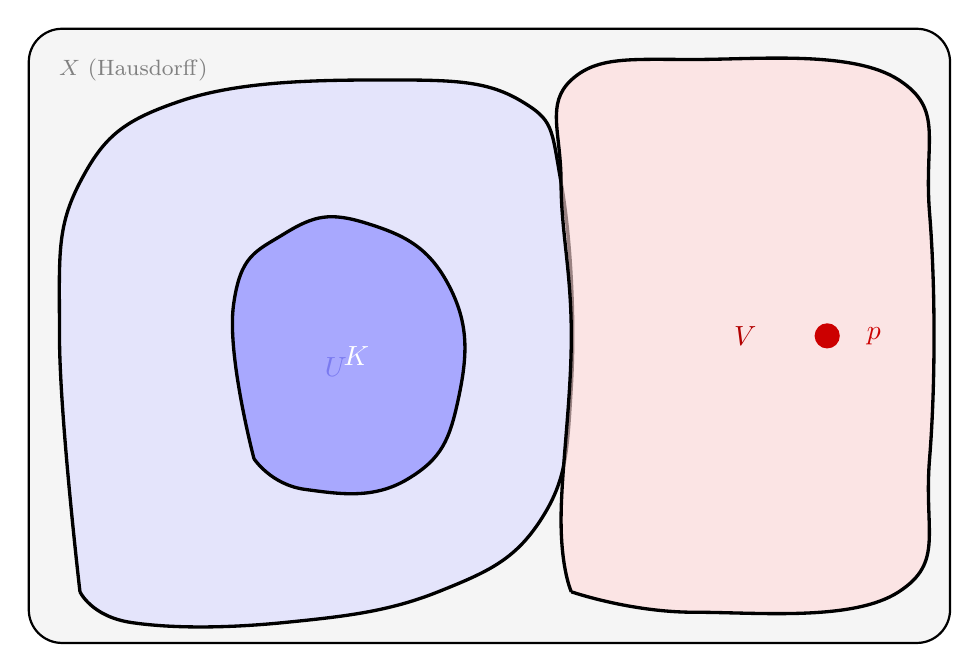
\begin{tikzpicture}[scale=1.3, every node/.style={font=\small}]
    % Espacio X como un rectángulo grande
    \draw[thick, rounded corners=12pt, fill=gray!8] (-4.5,-3) rectangle (4.5,3);
    \node[anchor=north west, font=\footnotesize, gray] at (-4.3, 2.8) {$X$ (Hausdorff)};

    % Abierto U con forma orgánica (izquierda)
    \begin{scope}
        \draw[very thick, fill=blue!15, fill opacity=0.6]
            plot[smooth, tension=0.7] coordinates {
                (-4.0, -2.5) (-3.5, -2.8) (-2.0, -2.8) (-0.5, -2.5)
                (0.5, -1.8) (0.8, -0.5) (0.7, 1.5) (0.3, 2.3)
                (-1.0, 2.5) (-3.0, 2.3) (-4.0, 1.5) (-4.2, 0) (-4.0, -2.5)
            };
    \end{scope}
    \node[font=\bfseries, text=blue!70!black] at (-1.5, -0.3) {$U$};

    % Conjunto compacto K dentro de U
    \begin{scope}
        \draw[very thick, fill=blue!40, fill opacity=0.8]
            plot[smooth, tension=0.8] coordinates {
                (-2.3, -1.2) (-1.8, -1.5) (-0.8, -1.4) (-0.3, -0.6)
                (-0.4, 0.5) (-1.2, 1.1) (-2.0, 1.0) (-2.5, 0.3) (-2.3, -1.2)
            };
    \end{scope}
    \node[font=\bfseries, text=white] at (-1.3, -0.2) {$K$};

    % Abierto V con forma orgánica (derecha)
    \begin{scope}
        \draw[very thick, fill=red!15, fill opacity=0.6]
            plot[smooth, tension=0.7] coordinates {
                (0.8, -2.5) (2.0, -2.7) (4.0, -2.5) (4.3, -1.2)
                (4.3, 1.2) (4.0, 2.5) (2.0, 2.7) (0.8, 2.5)
                (0.7, 1.5) (0.8, 0) (0.7, -1.8) (0.8, -2.5)
            };
    \end{scope}
    \node[font=\bfseries, text=red!70!black] at (2.5, 0) {$V$};

    % Punto p dentro de V
    \fill[red!80!black] (3.3, 0) circle (3.5pt);
    \node[anchor=west, font=\bfseries, text=red!80!black, inner sep=3pt] at (3.6, 0) {$p$};
\end{tikzpicture}
\end{center}
\begin{proof}
    Como X es de Hausdorff y $p \notin K$, para cada $x \in K$ existen abiertos disjuntos $U_x$ y $V_x$ tales que 
    $$x \in U_x,\quad p \in V_x, \quad U_x \cap V_x = \emptyset$$
    La familia $\{U_x\}_{x \in K}$ es un recubrimiento abierto de $K$. Como $K$ es compacto, existen $x_1, \ldots, x_n \in K$ tales que
    $$K \subset U_{x_1} \cup \ldots \cup U_{x_n}$$
    Definamos los conjuntos
    $$U = U_{x_1} \cup \ldots \cup U_{x_n}, \quad V = V_{x_1} \cap \ldots \cap V_{x_n}$$
    $U$ es abierto por ser unión numerable de finitos, y $V$ es abierto por ser intersección finita de abiertos. 
    Además, tenemos que $K \subset U$, ya que es construcción de un sobrecubrimiento finito de $K$. Por otro lado, $p \in V$ ya que $p \in V_{x_i}$ para cada $i = 1, \ldots, n$. Por último, $U \cap V = \emptyset$, ya que, dado $z \in U \implies z \in U_{x_i}$ para algún $i$, entonces $z \notin V_{x_i}$, lo que implica que $z \notin V$. Por lo tanto, $U$ y $V$ son abiertos disjuntos en $X$ tales que $K \subset U$ y $p \in V$.
\end{proof}
\begin{corolario}
    Todo subconjunto compacto de un espacio de Hausdorff es cerrado.
\end{corolario}
\begin{proof}
    Por la proposición anterior de separación de compactos en Hausdorff, dado un subconjunto compacto $K$ de un espacio de Hausdorff $X$, para cada punto $p \in X \setminus K$ podemos tomar $U, V \in \tau_X$ tales que $U \cap V = \emptyset$ y $K \subset U$ y $p \in V$. Por tanto, para cada $p \in X \setminus K$ existe un abierto $V_i$ tal que $p \in V_i \subset X \setminus K$, por lo tanto podemos ver que: 
    $$X \setminus K = \bigcup_{p \in X \setminus K} V_p$$
    lo que implica que $X \setminus K$ es abierto, por lo tanto $K$ es cerrado.
\end{proof}
\begin{proposición}
    Si $X$ es un espacio de Hausdorff, entonces la intersección de subconjuntos compactos es compacta.
\end{proposición}
\begin{proof}
    Sea una sucesión finita de subconjuntos de $X$ compactos, $K_i$. Por ser compactos en un espacio de Hausdorff, cada uno de los $K_i$ es cerrado. Por lo que $\cap_{i = 1}^{n} K_i = K$ es un conjunto cerrado. Y dado que $K \subset K_i \forall i$, entonces $K$ es compacto por ser subconjunto cerrado de un compacto.
\end{proof}
\ejemplo{
    Obtén los compactos de $\mathbb{R}$ con la topología de Kolmogorov: 
    $$\tau_k = \{\emptyset, \mathbb{R}\} \cup \{(-\infty, a) : a \in \mathbb{R}\}$$
    Según como está definida la topología, la unión arbitraria de una sucesión de abiertos básicos $(- \infty, - a_i)_{i \in \mathbb{N}}$ es un abierto de $\tau_k$ y su unión viene dada por $(- \infty, \max{a_i}_{i \in \mathbb{N}})$. Por lo tanto, para cada conjunto definido en $\mathbb{R}$, podemos definir un recubrimiento abierto de $\tau_k$ pero siempre será un intervalo de la forma $(-\infty, a)$. \\
    En este caso, podemos distinguir dos casos: 
    \begin{enumerate}
        \item Si $K$ está acotado superiormente: Sea $M = \sup K$. Entonces, si consieramos el recubrimiento abierto $\{(-\infty, M + \frac{1}{n}) : n \in \mathbb{N}\}$, entonces $K \subset (-\infty, M + \frac{1}{N})$ para algún $N$, que contiene a $K$. Funciona, así que no hay problema. Pero si $M \notin K$, el recubrimiento $\{(- \infty, M)\}$ ya cubre $K$, por ser $M$ supremo. 
        \item Si $K$ no está acotado superiormente: En este caso, el recubrimiento $\{(-\infty, n) : n \in \mathbb{N}\}$ cubre a $K$, pero no existe ningún recubrimiento finito de este tipo que cubra a $K$, ya que para cada $n$ existe un elemento de $K$ mayor que $n$. Por lo tanto, $K$ no es compacto.
    \end{enumerate}
}
\ejemplo{
    Obtén los compactos de $\mathbb{R}$ con la topología cofinta: 
    $$\tau_c = \{\emptyset\} \cup \{A \subset \mathbb{R} : \mathbb{R} \setminus A \text{ es finito}\}$$
    Sea $K \subset \mathbb{R}$ un candidato a compacto, y sea $\{U_i\}_{i \in \mathcal{I}}$ un recubrimiento abierto de $K$. Si tomamos uno de los abiertos del recubrimiento, digamos $U_{i_0}$ entonces, por definición de la topología $X \setminus U_{i_0} = \{x_1, \ldots, x_n\}$. Entonces, si tomamos el conjunto $V = \{x_1, \ldots, x_n\} \cap K$ que es un conjunto finito, podemos tomar los abiertos del recubrimiento original que los contienen, de manera que $x_i \in U_{i}$ y por tanto, tenemos que
    $$K \subset U_{i_0} \cup U_{i_1} \cup \ldots \cup U_{i_n}$$
}
\ejemplo{
    Obtén los compactos de $\mathbb{R}$ con la topología conumerable:
    $$\tau_{con} = \{\emptyset\} \cup \{A \subset \mathbb{R} : \mathbb{R} \setminus A \text{ es numerable} \}$$
    Dado que dentro de la categoría de conjuntos numerables se encuentran los conjuntos finitos, el argumento para la topología cofinta también funciona para esta topología, por lo que todo conjunto de $\mathbb{R}$ finito es compacto.

    No obstante, esto no ocurre para los conjuntos numerables infinitos. Tomemos de ejemplo al conjunto de los naturales $\mathbb{N}$. Un recubrimiento abierto de este conjunto sería la familia:
    $$\{U_n : n \in \mathbb{N}\} \quad \text{donde} \quad U_n = \mathbb{R} \setminus (\mathbb{N} \setminus \{n\})$$
    ya que $\mathbb{N} \setminus \{n\}$ es un conjunto numerable, por lo que $U_n$ es abierto en $\tau_{con}$. Sin embargo, de este recubrimiento no puede obtenerse ningún subrecubrimiento abierto y finito, pues cada $U_n$ cubre solamente a los puntos excepto a un conjunto numerable. Por lo tanto, $\mathbb{N}$ no es compacto. Y dado que la compacidad es una propiedad topológica (es decir, que se conserva bajo homeomorfismos), ningún conjunto numerable infinito es compacto en $\tau_{con}$.
}
\ejemplo{
    Obtén los compactos de $X = \{\mathbb{R}^2 \setminus \{(0,0)\} \}$ con la topología que tiene por base al conjunto 
    $$\beta = \{(tx, ty) : 0 \leq t \leq 1, (x,y) \in X\} = \{(R, \theta) : R > 0, \theta \in [0, 2\pi)\}$$
    Dado que dado un rayo $(R, \theta)$, la unión de los rayos con el mismo ángulo $\theta$ es un abierto de la topología, entonces cada rayo es un abierto de la topología. \\
    Podemos intuir entonces que un conjunto $K$ sólo podría ser compacto en caso de que tenga un numero finito de puntos de distintas angulaciones, ya que si tuviera un número infinito de puntos con distintas ángulos, entonces podríamos construir un recubrimiento abierto de $K$ formado por los rayos que contienen a cada uno de estos puntos, y no existiría ningún subrecubrimiento finito de este tipo. \\
    Además, cada uno de los rayos debe tener un máximo, pues en caso contrario, no estaría acotado y no sería posible obtener un recubrimiento finito de un subrecubrimiento. 
    Por lo tanto, los compactos de $X$ con esta topología son exactamente los conjuntos finitos de puntos de $X$.
}
\ejemplo{
    Obtén los compactos de $X$ con la topología definida por $$\tau = \{\emptyset\} \cup \{U \subset X : A \subset U\}$$
    siendo $A \subset X$ fijo tal que $A \neq \emptyset$. 
    Podemos disntiguinir dos casos: 
    \begin{enumerate}
        \item $A \not\subseteq K$: En este caso $K$ no contiene a $A$ completo, por lo que $K$ no es abierto. Para formar un recubrimiento debemos tomar conjuntos $U$ tales que deben contener a $A$, en particular deben contener los puntos de $A$ que no están en $K$. Así, tomamos el recubrimiento de $K$: 
        $$\mathcal{U} = \{A \cup \{x\} : x \in K \setminus A\} \cup \{A\}$$
        El cual es abierto ya que $A \subset A \cup \{x\}$. Para poder obtener un sobrecubrimiento finito de este recubrimiento, debemos cubrir todos los puntos de $K \setminus A$ con un número finito de conjuntos de la forma $A \cup \{x\}$, lo que requiere que $K \setminus A$ sea finito. 
        \item $A \subseteq K$: En este caso, podemos tomar un recubrimiento de $K$ parecido al anterior, 
        $$\mathcal{V} = \{A \cup \{x\} : x \in K \setminus A \}$$ 
        El cual recubrie $K$ porque recubre los puntos de $A$ que están cubrietos por cualquier elemento de $\mathcal{V}$, y cada uno de los puntos de $K \setminus A$ está cubierto por el conjunto $A \cup \{x\}$ que lo contiene. No obstante, si $K \setminus A$ es infinito, entonces no existe ningun sobrecubrimiento finito, por lo que $K$ no es compacto. Por lo tanto, $K$ es compacto si y sólo si $K \setminus A$ es finito.
    \end{enumerate}
}
\begin{proposición}
    Dado un subconjunto $K \subset X$ compacto, entonces: 
    \begin{enumerate}
        \item $Int(K)$ es compacto.
        \item $X$ es un espacio de Hausdorff $\implies \overline{K}$ es compacto.
        \item $X$ es un espacio de Hausdorff $\implies \partial K = \overline{K} \setminus Int(K) = \overline{K} \cap \overline{X \setminus K}$ es compacto.
        \item $X$ es un espacio de Hausdorff $ \implies K^{\prime}$ es compacto.
    \end{enumerate}
\end{proposición}
\begin{proof}
    \begin{enumerate}
        \item Sabemos que $Int(K) \subset K$, por lo tanto, si para $K$ se puede obtener un recubrimiento finito de todo sobrecubrimiento abierto, entonces para $Int(K)$ también se puede obtener un recubrimiento finito de todo sobrecubrimiento abierto, ya que cada recubrimiento abierto de $Int(K)$ es también un recubrimiento abierto de $K$. Por lo tanto, $Int(K)$ es compacto.
        \item Como $K$ es compacto y $X$ es un espacio de Hausdorff, entonces $K$ es cerrado, por lo que $\overline{K} = K$, lo que implica que $\overline{K}$ es compacto. 
        \item Dado que $\partial(K) = \overline{K} \cap \overline{X \setminus K}$, entonces es un conjunto cerrado y como $\partial(K) \subset \overline{K}$ y $\overline{K}$ es compacto, entonces $\partial(K)$ es un subconjunto cerrado de un compacto, por lo que $\partial(K)$ es compacto.
        \item Si $X$ es de Hausdorff, entonces $K^{\prime} \subset K$ es un subconjunto cerrado de un compacto, por lo que $K^{\prime}$ es compacto.
    \end{enumerate} 
\end{proof}
\begin{proposición}
    Si $X$ es un espacio de Hausdorff y $A, B \subset X$ son dos subconjuntos compactos y disjuntos de $X$, entonces existen abiertos $U$ y $V$ abiertos disjuntos en $X$ tales que $A \subset U$ y $B \subset V$.
\end{proposición}
\begin{proof}
    $X$ es un espacio de Hausdorff $\iff \forall x, y \in X \exists U, V \in \tau : U \cap V = \emptyset, x \in U, y \in V$. \\
    Sean $A,B \subset X : A \cap B = \emptyset$ dos subconjuntos compactos de $X$. Ahora tomemos $x \in X \setminus B$ y para cada $b \in B$ como $X$ es de Hausdorff, existen abiertos disjuntos $U_b$ y $V_b$ tales que $x \in U_b$, $b \in V_b$ y $U_b \cap V_b = \emptyset$. La familia $\{V_b : b \in B\}$ es un recubrimiento abierto de $B$, por lo que existen $b_1, \ldots, b_n \in B$ tales que: 
    $$B \subset V_{b_1} \cup \ldots \cup V_{b_n}$$
    Tomando $U_X = \bigcap_{i = 1}^{n} U_{b_i}$ y $V_X = V_{b_1} \cup \ldots \cup V_{b_n}$, entonces $U_X$ y $V_X$ son abiertos y $U_X \cap V_X = \emptyset$. Así, hemos separado el conjunto compacto $B$ de un punto $x$. \\
    Ahora para el compacto $A$, para cada $a \in A$ tomamos $U_a$ y $V_a$ tales que $a \in U_a$, $B \subset V_a$. Como la familia $\{U_a : a \in A\}$ es un recubrimiento abierto de $A$, entonces existen $a_1, \ldots, a_m \in A$ tales que:
    $$ A \subset U = U_{a_1} \cup \ldots \cup U_{a_m}$$
    Tomando 
    $$V = \bigcap_{i = 1}^{m} V_{a_i}$$
    entonces $V$ es un abierto que contiene a $B$ y $U \cap V = \emptyset$. Por lo tanto, $U$ y $V$ son abiertos disjuntos en $X$ tales que $A \subset U$ y $B \subset V$.
\end{proof}
\begin{definición}[Espacio normal o $T_4$]
    Un espacio topológico $(X, \tau)$ es un espacio $T_4$ si para cada par de subconjuntos cerrados disjuntos $A, B \subset X$ existen abiertos disjuntos $U$ y $V$ tales que $A \subset U$ y $B \subset V$.
\end{definición}
\begin{corolario}
    Todo espacio compacto y de Hausdorff es un espacio normal, es decir, es un espacio $T_4$.
\end{corolario}
\begin{definición}[Primero numerable]
    Un espacio topológico $(X, \tau)$ es primero numerable si cada punto $x \in X$ tiene una base numerable de entornos.
\end{definición}
\begin{definición}[Segundo numerable]
    Un espacio topológico $(X, \tau)$ es segundo numerable si tiene una base numerable para su topología.
\end{definición}
\begin{definición}[Espacio de Lindelöf]
    Un espacio topológico $(X, \tau)$ es un espacio de Lindelöf si todo recubrimiento abierto de $X$ admite un subrecubrimiento numerable. Es decir, 
    $$\forall \mathcal{U} \subset \tau : X \subset \bigcup \mathcal{U} \Rightarrow \exists \mathcal{V} \subset \mathcal{U} \text{ numerable } : X \subset \bigcup \mathcal{V}$$
    
\end{definición}
\begin{teorema}[Teorema de Lindelöf]
    Si $X$ es un espacio topológico segundo numerable, todo recubrimiento abierto de $X$ admite un subrecubrimiento numerable.
\end{teorema}
\begin{proof}
    Sea $\mathcal{B} = \{B_n\}_{n \in \mathbb{N}}$ una base numerable de $\tau$, y sea $\{U_i\}_{i \in \mathcal{I}}$ un recubrimiento abierto de $X$. Para cada $x \in X$ existe algún $U_i$ con $x \in U_i$. Como $\mathcal{B}$ es una base, existe algún $B_n$ tal que $x \in B_n \subset U_i$. Definamos 
    $$\mathcal{J} = \{n \in \mathbb{N} : \exists i \in \mathcal{I} : B_n \subset U_i\}$$
    Entonces $\{B_n : n \in \mathcal{J}\}$ es un recubrimiento abierto de $X$ formado por elementos de la base. Además, $\mathcal{J} \subset \mathbb{N}$ por lo que como máximo es numerable. \\
    Para cada $n \in \mathcal{J}$ elegimos un $i(n) \in \mathcal{I}$ tal que $B_n \subset U_{i(n)}$. Entonces, 
    $$X = \bigcup_{n \in \mathcal{J}} B_n \subset \bigcup_{n \in \mathcal{J}} U_{i(n)}$$
    Así, $\{U_{i(n)} : n \in \mathcal{J}\}$ es un subrecubrimiento numerable de $\{U_i\}_{i \in \mathcal{I}}$.
\end{proof}
\begin{definición}[Espacio separable]
    Un espacio topológico $(X, \tau)$ es separable si existe un subconjunto denso de $X$ que sea numerable. Es decir, existe $A \subset X$ tal que $A$ es numerable y $\overline{A} = X$.
    
\end{definición}
\begin{proposición}
    Si $X$ es un espacio metrizable y compacto o de Lindelöf, entonces $X$ es separable y por tanto segundo numerable.
\end{proposición}
\begin{proof}
    Sea $d$ la métrica de $X$. Para cada $n \in \mathbb{N}$, consideramos el recubrimiento abierto: 
    $$\left\{B(x, \frac{1}{n})\right\}_{x \in X}$$
    Como $X$ es de Lindelöf, existe un subrecubrimiento numerable de este recubrimiento, es decir, fijado un $n \in \mathbb{N}$ existe una sucesión $\{x_{n, k}\}_{k \in \mathbb{N}}$ de puntos de $X$ tal que:
    $$X = \bigcup_{k \in \mathbb{N}} B\left(x_{n, k}, \frac{1}{n}\right)$$
    Definimos $D = \{x_{n, k} : n, k \in \mathbb{N}\}$, que es unión numerable de conjuntos numerables, luego es numerable. Y $D$ es denso: dado $x \in X$ y $\varepsilon > 0$, tomamos $n$ con $\frac{1}{n} < \varepsilon$ y existe algún $x_{n, k}$ con $x \in B(x_{n, k}, \frac{1}{n})$, es decir, 
    $$d(x, x_{n, k}) < \frac{1}{n} < \varepsilon$$
    Así, $D$ es un subconjunto denso y numerable, y por tanto $X$ es separable. 
\end{proof}
\begin{proposición}
    Si $X$ es compacto y $f: X \to Y$ es continua y sobreyectiva, entonces $Y$ es compacto.     
\end{proposición}
\begin{proof}
    Dado un recubrimiento $\{U_i\}_{i \in \mathbb{N}}$ de $Y$, como $f: X \to Y$ es continua, esto implica que $f^{-1}(U_i) \in \tau_X$, entonces, tenemos que
    $$ Y = \bigcup_{n \in \mathbb{N}} U_n \implies f^{-1}(Y) = f^{-1}\left(\bigcup_{n \in \mathbb{N}} U_n\right) = X = \bigcup_{n \in \mathbb{N}} f^{-1}(U_n) \in \tau_X$$
    Luego $\{f^{-1}(U_n) : n \in \mathbb{N}\}$ es un recubrimiento abierto de $X$. Por la compacidad de $X$, existe un subrecubrimiento finito $\{f^{-1}(U_{n_1}), \ldots, f^{-1}(U_{n_k})\}$ de $X$. Por lo tanto, ahora aplicando $f$ nuevamente, 
    $$Y = f(X) = f\left(\bigcup_{i = 1}^{k} f^{-1}(U_{n_i})\right) = \bigcup_{i = 1}^{k} U_{n_i}$$, lo que demuestra que $Y$ es compacto. 
\end{proof}
\begin{corolario}
    \vspace{-1 cm} 
    \begin{enumerate}
        \item Si $f: X \to Y$ es continua y $K \subset X$ es compacto, entonces $f(K)$ es compacto.
        \item La compacidad es una propiedad topológica, es decir, si $X$ y $Y$ son espacios homeomorfos, entonces $X$ es compacto si y sólo si $Y$ es compacto.
        \item Todo espacio cociente de un espacio compacto es compacto.
    \end{enumerate}
\end{corolario}
\begin{definición}[Topología final]
    La topología final para la aplicación $f: (X, \tau_X) \to (Y, \tau_Y)$ es la topología más fina en $Y$ que hace continua a $f$. Es decir, $\tau_Y = \{U \subset Y : f^{-1}(U) \in \tau_X\}$.
\end{definición}
\begin{definición}[Identificación]
    Una aplicación $f: X \to Y$ entre espacios topológicos es una\textbf{identificación} si:
    \begin{enumerate}
        \item $f$ es continua
        \item $f$ es sobreyectiva
        \item La topología de $Y$ es la topología final para $f$
    \end{enumerate}
\end{definición}
\begin{proposición}
    Sea $f:X \to Y$ una aplicación continua y sobreyectiva. Entonces, $f$ es una identificación si:
    \begin{enumerate}
        \item $f$ es cerrada
        \item $f$ es abierta
        \item $f$ admite una sección continua, es decir, existe una aplicación continua $s:Y \to X$ talque $f \circ s = id_Y$.
    \end{enumerate}
\end{proposición}
\begin{definición}[Homeomorfismo]
    Una aplicación $f: X \to Y$ entre espacios topológicos es un homeomorfismo si:
    \begin{enumerate}
        \item $f$ es continua
        \item $f$ es biyectiva
        \item La aplicación inversa $f^{-1}: Y \to X$ es continua
    \end{enumerate}
\end{definición}
\begin{proposición}
    Sea $X$ un espacio compacto, $Y$ un espacio Hausdorff y $f: X \to Y$ una aplicación continua. Entonces: 
    \begin{enumerate}
        \item $f$ es cerrada
        \item Si $f$ es sobreyectiva, entonces $f$ es una identificación.
        \item Si $f$ es biyectiva, entonces $f$ es un homeomorfismo.
        \item Es necesario que $Y$ sea de Hausdorff para que se cumplan esas propiedades. 
    \end{enumerate}
\end{proposición}
\begin{proof}
    \begin{enumerate}
        \item $f$ es cerrada $\iff \forall A \subset X : A \text{ cerrado} \implies f(A) \text{ cerrado}$. Dado $A  \subset X$ cerrado, como $X$ es compacto, entonces $A$ es compacto. Por lo tanto como la función es continua, entonces $f(A)$ es compacto. Y como $Y$ es de Hausdorff, entonces $f(A)$ es cerrado. Por lo tanto, $f$ es cerrada.
        \item Sabemos que $f$ es continua y sobreyectiva, como por el apartado anterior $f$ es cerrada, entonces $f$ es una identificación.
        \item Por el apartado anterior, como $f$ es cerrada, entonces $f$ es una identificación. Además, como $f$ es biyectiva, entonces $f^{-1}: Y \to X$ es una aplicación continua, lo que implica que $f$ es un homeomorfismo.
        \item Si $Y$ no es de Hausdorff, entonces no se cumple el primer apartado, por lo que no se cumplen los apartados siguientes. Por lo tanto, es necesario que $Y$ sea de Hausdorff para que se cumplan esas propiedades.
    \end{enumerate}  
\end{proof}
\begin{proposición}
    Si $X$ es un espacio compacto y de Hausdorff y $f: X \to Y$ es sobreyectiva, continua y cerrada, entonces $Y$ es un espacio de Hausdorff y compacto.
\end{proposición}
\begin{proof}
    Dado que $f$ es una aplicación continua por hipótesis, entonces $f(X) = Y$ (por sobreyectividad) es un compacto. \\
    Para demostrar que $Y$ es de Hausdorff, tomemos $y_1, y_2 \in Y$ con $y_1 \neq y_2$. Consideremoslas fibras de $y_1$ y $y_2$:
    $$f^{-1}(y_1) = \{x \in X : f(x) = y_1\}, \quad f^{-1}(y_2) = \{ x \in X : f(x) = y_2\}$$
    Las fibras son cerradas y disjuntas por la continuidad de $X$. Como $X$ es de Hausdorff y compacto, las fibras son compactos y disjuntos, podemos separar cada par de puntos $x_1 \in f^{-1}(y_1)$ y $x_2 \in f^{-1}(y_2)$ con abiertos disjuntos. Por compacidad de ambasibras, existen abiertos disjuntos $U, V \subset X$ con
    $$f^{-1}(y_1) \subset U, \quad f^{-1}(y_2) \subset V$$
    Ahora definimos
    $$W_1 = Y \setminus f(X \setminus U), \quad W_2 = Y \setminus f(X \setminus V)$$
    Como $X \setminus U$ y $X \setminus V$ son cerrados, entonces $W_1$ y $W_2$ son abiertos.
    \begin{itemize}
        \item $y_1 \in W_1$: pues $f^{-1}(y_1) \subset U$, luego $f^{-1}(y_1) \cap (X \setminus U) = \emptyset$ es decir, $y_1 \notin f(X \setminus U)$, por lo que $y_1 \in W_1$.
        \item $y_2 \in W_2$: análogamente
        \item $W_1 \cap W_2 = \emptyset$: si $y \in W_1 \cap W_2$, entonces $y \in W_1$ y $y \in W_2$, lo que implica que $y \notin f(X \setminus U)$ y $y \notin f(X \setminus V)$. Por lo tanto, $f^{-1}(y) \subset U \cap V = \emptyset$, lo cual es una contradicción. Por lo tanto, $W_1 \cap W_2 = \emptyset$. 
    \end{itemize}
\end{proof}
\begin{proposición}
    Si $X$ es compacto, y $f: X \to \mathbb{R}$ es continua, entonces $f$ no es abierta y alcanza su máximo y su mínimo.
\end{proposición}
\begin{proof}
    Como $X$ es compacto y $f$ es continua, entonces $f(X)$ es compacto en $\mathbb{R}$, por lo que $f(X)$ es cerrado y acotado. Por lo tanto, $f(X)$ tiene un máximo y un mínimo, que son elementos de $f(X)$, por lo que existen $x_{max}, x_{min} \in X$ tales que $f(x_{max}) = \max f(X)$ y $f(x_{min}) = \min f(X)$. \\

\end{proof}
\begin{proposición}[Proyección cerrada]
    Si $Y$ es compacto, la proyección $\pi: X \times Y \to X$ es cerrada.
\end{proposición}
\begin{proof}
    %TODO
\end{proof}
\begin{lema}[Lema del tubo]
    Sean $x \in X$ y $U$ un abierto de $X \times Y$ tales que $\{x\} \times Y \subset U$. Si $Y$ es compacto, existe $V$ abierto de $X$ tal que $x \in V$ y $V \times Y \subset U$.
\end{lema}
\begin{proof}
    %TODO
\end{proof}
\begin{proposición}[Compacidad del producto finito]
    Si $X$ e $Y$ son espacios topológicos compactos, $X \times Y$ es compacto.
\end{proposición}
\begin{proof}
    %TODO
\end{proof}
\begin{teorema}[Teorema de Tijonov]
    Un espacio producto es compacto si, y sólo si, lo son todos sus factores.
\end{teorema}
\begin{proof}
    %TODO
\end{proof}
\begin{lema}[Lema de Lebesgue]
    Si $\mathcal{U}$ es una cobertura abierta de un espacio métrico compacto $(M, d)$, existe $\varepsilon > 0$, llamado número de Lebesgue de $\mathcal{U}$, tal que todo subconjunto de diámetro menor que $\varepsilon$ está contenido en algún elemento de $\mathcal{U}$.
\end{lema}
\begin{proof}
    %TODO
\end{proof}
\begin{proposición}[Continuidad uniforme]
    Toda aplicación continua entre espacios métricos con dominio compacto es uniformemente continua.
\end{proposición}
\begin{proof}
    %TODO
\end{proof}
\begin{teorema}[Caracterización de la compacidad en espacios métricos]
    Para cualquier espacio métrico $M$ son equivalentes:
    \begin{enumerate}
        \item $M$ es compacto.
        \item Todo subconjunto infinito de $M$ tiene un punto de acumulación (propiedad de Bolzano-Weierstrass).
        \item Toda sucesión en $M$ tiene una subsucesión convergente (compacidad secuencial).
        \item $M$ es completo y toda sucesión en $M$ tiene una subsucesión de Cauchy (totalmente acotado).
    \end{enumerate}
\end{teorema}
\begin{proof}
    %TODO
\end{proof}

\subsection{Compacidad local}

\begin{definición}[Localmente compacto]
    Un espacio topológico $(X, \tau)$ es localmente compacto cuando todo punto de $X$ tiene una base local de vecindades compactas.
\end{definición}
\begin{corolario}
    Todo espacio compacto y de Hausdorff es localmente compacto.
\end{corolario}
\begin{proof}
    %TODO
\end{proof}
\begin{proposición}[Caracterización en espacios de Hausdorff]
    Un espacio de Hausdorff $X$ es localmente compacto si, y sólo si, cada punto de $X$ tiene una vecindad compacta.
\end{proposición}
\begin{proof}
    %TODO
\end{proof}
\begin{proposición}
    Si $X$ es un espacio localmente compacto e $Y \subset X$ es un subespacio abierto o cerrado de $X$, entonces $Y$ es localmente compacto.
\end{proposición}
\begin{proof}
    %TODO
\end{proof}
\begin{proposición}
    Si $Y \subset X$ es un subespacio localmente compacto de un espacio de Hausdorff $X$, entonces $Y$ es intersección de un abierto y un cerrado de $X$.
\end{proposición}
\begin{proof}
    %TODO
\end{proof}
\begin{proposición}
    Si $X$ es localmente compacto y $f: X \to Y$ es sobreyectiva, continua y abierta, entonces $Y$ es localmente compacto.
\end{proposición}
\begin{proof}
    %TODO
\end{proof}
\begin{corolario}
    La compacidad local es una propiedad topológica.
\end{corolario}
\begin{proof}
    %TODO
\end{proof}
\begin{proposición}[Producto de localmente compactos]
    $X \times Y$ es localmente compacto si, y sólo si, $X$ e $Y$ son localmente compactos.
\end{proposición}
\begin{proof}
    %TODO
\end{proof}
\begin{teorema}[Teorema de Whitehead]
    Si $f: X \to Y$ es una identificación y $Z$ es un espacio localmente compacto, entonces $f \times \mathrm{Id}_Z: X \times Z \to Y \times Z$ es una identificación.
\end{teorema}
\begin{proof}
    %TODO
\end{proof}

\subsection{Compactificación}

\begin{definición}[Compactificación]
    Una compactificación de un espacio topológico $X$ es un par $(K, \varphi)$ donde $K$ es un espacio topológico compacto y $\varphi: X \to K$ es un mergullimiento (embedding) tal que $\varphi(X)$ es denso en $K$. Si $K$ es de Hausdorff, se dice que $(K, \varphi)$ es una compactificación Hausdorff de $X$.
\end{definición}
\begin{definición}[Compactificaciones equivalentes]
    Dos compactificaciones $(K, \varphi)$ y $(L, \psi)$ de un espacio $X$ son (topológicamente) equivalentes si existe un homeomorfismo $h: K \to L$ tal que $h \circ \varphi = \psi$.
\end{definición}
\begin{definición}[Compactificación de Aleksandrov]
    Sea $(X, \tau)$ un espacio topológico y $\infty \notin X$. Se define $X^* = X \cup \{\infty\}$ y
    $$\tau^* = \tau \cup \{A \subset X^* : X^* \setminus A \text{ es cerrado y compacto en } (X, \tau)\}.$$
\end{definición}
\begin{proposición}
    $(X^*, \tau^*)$ es un espacio topológico compacto que contiene a $(X, \tau)$ como subespacio.
\end{proposición}
\begin{proof}
    %TODO
\end{proof}
\begin{proposición}
    Si $j: X \hookrightarrow X^*$ es la inclusión, entonces $(X^*, j)$ es compactificación de $X$ si, y sólo si, $X$ no es compacto.
\end{proposición}
\begin{proof}
    %TODO
\end{proof}
\begin{proposición}
    La compactificación de Aleksandrov de un espacio no compacto $X$ es Hausdorff si, y sólo si, $X$ es Hausdorff y localmente compacto.
\end{proposición}
\begin{proof}
    %TODO
\end{proof}
\begin{proposición}
    Sean $X$ e $Y$ espacios no compactos, localmente compactos y de Hausdorff, y $f: X \to Y$ una aplicación continua. Denótese por $f^*: X^* \to Y^*$ a la extensión de $f$ a las compactificaciones de Aleksandrov definida por $f^*(\infty_X) = \infty_Y$ y $f^*(x) = f(x)$ para todo $x \in X$. Entonces $f^*$ es continua si, y sólo si, $f$ es propia.
\end{proposición}
\begin{proof}
    %TODO
\end{proof}
\begin{proposición}
    Sea $X$ no compacto, localmente compacto y de Hausdorff. Si $(K, \varphi)$ es una compactificación Hausdorff de $X$ tal que $K \setminus \varphi(X)$ es unitario, entonces $(K, \varphi)$ es equivalente a la compactificación de Aleksandrov de $X$.
\end{proposición}
\begin{proof}
    %TODO
\end{proof}
\begin{proposición}
    Sea $X$ un espacio no compacto, localmente compacto y de Hausdorff. Para cada compactificación Hausdorff $(K, \varphi)$ de $X$ existe una aplicación sobreyectiva y continua $h: K \to X^*$ tal que $h \circ \varphi = j$. Además, la compactificación de Aleksandrov $X^*$ es la única (salvo equivalencias) que verifica esta propiedad.
\end{proposición}
\begin{proof}
    %TODO
\end{proof}